%%%%%%%%%%%%%%%%%%%%%%%%%%%%%%%%%%%%%%%%%%%%%%
%                                            %
%   W Z O R Z E C   S P R A W O Z D A N I A  %
%                                            %
%%%%%%%%%%%%%%%%%%%%%%%%%%%%%%%%%%%%%%%%%%%%%%


\documentclass[12pt,a4paper]{article}

\usepackage{amsmath,amssymb}
\usepackage[utf8]{inputenc}                                      
\usepackage[OT4]{fontenc}      
%\usepackage[T1]{fontenc}                            
\usepackage[polish]{babel}                           
\selectlanguage{polish}
\usepackage{indentfirst} 
\usepackage[dvips]{graphicx}
\usepackage{tabularx}
\usepackage{color}
\usepackage{hyperref} 
\usepackage{fancyhdr}
\usepackage{listings}
\usepackage{booktabs}
\usepackage{ifpdf}
\usepackage{mathtext} % polskie znaki w trybie matematycznym
%\makeindex  % utworzenie skorowidza (w dokumencie pdf)
\usepackage{lmodern}
%\usepackage[osf]{libertine}
\usepackage{filecontents}
\usepackage{ifthen}

\usepackage{graphicx}
\graphicspath{ {./pics/} }

\usepackage{tikz}
\usetikzlibrary{arrows}


\newcounter{nextYear}
\setcounter{nextYear}{\the\year}
\stepcounter{nextYear}

% rozszerzenie nieco strony
\setlength{\topmargin}{-1cm} \setlength{\textheight}{24.5cm}
\setlength{\textwidth}{17cm} \addtolength{\hoffset}{-1.5cm}
\setlength{\parindent}{0.5cm} \setlength{\footskip}{2cm}
\linespread{1.2} % odstep pomiedzy wierszami


%%%% ZYWA PAGINA %%%%%%%%%%%
\newcommand{\tl}[1]{\textbf{#1}} 
\pagestyle{fancy}
\renewcommand{\sectionmark}[1]{\markright{\thesection\ #1}}
\fancyhf{} % usuwanie bieżących ustawień
\fancyhead[LE,RO]{\small\bfseries\thepage}
\fancyhead[LO]{\small\bfseries\rightmark}
\fancyhead[RE]{\small\bfseries\leftmark}
\renewcommand{\headrulewidth}{0.5pt}
\renewcommand{\footrulewidth}{0pt}
\addtolength{\headheight}{0.5pt} % pionowy odstęp na kreskę
\fancypagestyle{plain}{%
\fancyhead{} % usuń p. górne na stronach pozbawionych numeracji
\renewcommand{\headrulewidth}{0pt} % pozioma kreska
}

%%%%%   LISTINGI %%%%%%%%
% ustawienia listingu programow

\lstset{%
language=C++,%
commentstyle=\textit,%
identifierstyle=\textsf,%
keywordstyle=\sffamily\bfseries, %
%captionpos=b,%
tabsize=3,%
frame=lines,%
numbers=left,%
numberstyle=\tiny,%
numbersep=5pt,%
breaklines=true,%
morekeywords={pWezel,Wezel,string,ref,params_result},%
escapeinside={(*@}{@*)},%
%basicstyle=\footnotesize,%
%keywords={double,int,for,if,return,vector,matrix,void,public,class,string,%
%float,sizeof,char,FILE,while,do,const}
}
%%%%%%%%%%%%%%%%%%%%%%%%%%%%%%%%%%%%%%%%%%%%%%%%%%%%%%%%%%%%%%%%%%%%%%%

%%%%%%%%%  NOTKI NA MARGINESIE %%%%%%%%%%%%%
% mala zmiana sposobu wyswietlania notek bocznych
\let\oldmarginpar\marginpar
\renewcommand\marginpar[1]{%
  {\linespread{0.85}\normalfont\scriptsize%
\oldmarginpar[\hspace{1cm}\begin{minipage}{3cm}\raggedleft\scriptsize\color{black}\textsf{#1}\end{minipage}]%    left pages
{\hspace{0cm}\begin{minipage}{3cm}\raggedright\scriptsize\color{black}\textsf{#1}\end{minipage}}% right pages
}%
}
% % % % % % % % % % % % % % % % % % % % % % % % % % % % % % % %

%%%% WYSWIETLANIE AKTUALNEGO ROKU AKADEMICKIEGO %%%%%%%%%%%
\newcounter{rok}
\newcommand{\rokakademicki}{%
   \setcounter{rok}{\number\year}%
   \ifthenelse{\number\month<10}%
   {\addtocounter{rok}{-1}}% rok akademicki zaczal sie w pazdzierniku poprzedniego roku
   {}%                       rok akademicki zaczyna sie w pazdzierniku tego roku
   \arabic{rok}/\addtocounter{rok}{1}\arabic{rok}
}
%%%%%%%%%%%%%%%%%%%%%%%%%%%%%%%%%%%%%%%


%%%% LISTA UWAG %%%%%%%%%
\usepackage{color}
\definecolor{brickred}      {cmyk}{0   , 0.89, 0.94, 0.28}

\makeatletter \newcommand \kslistofremarks{\section*{Uwagi} \@starttoc{rks}}
\newcommand\l@uwagas[2]
{\par\noindent \textbf{#2:} %\parbox{10cm}
   {#1}\par} \makeatother


\newcommand{\ksremark}[1]{%
   {{\color{brickred}{[#1]}}}%
   \addcontentsline{rks}{uwagas}{\protect{#1}}%
}

\newcommand{\comma}{\ksremark{przecinek}}
\newcommand{\nocomma}{\ksremark{bez przecinka}}
\newcommand{\styl}{\ksremark{styl}}
\newcommand{\ortografia}{\ksremark{ortografia}}
\newcommand{\fleksja}{\ksremark{fleksja}}
\newcommand{\pauza}{\ksremark{pauza `--', nie dywiz `-'}}
\newcommand{\kolokwializm}{\ksremark{kolokwializm}}
\newcommand{\cytowanie}{\ksremark{cytowanie}}

%%%%%%%%%%%%%%%%%%%%%%%%%
%%%%%%%%%%%%%%%%%%%%%%%%%
%%%%%%%%%%%%%%%%%%%%%%%%%
%%%%%%%%%%%%%%%%%%%%%%%%%
%%%%%%%%%%%%%%%%%%%%%%%%%
%%%%%%%%%%%%%%%%%%%%%%%%%
%%%%%%%%%%%%%%%%%%%%%%%%%
%%%%%%%%%%%%%%%%%%%%%%%%%
%%%%%%%%%%%%%%%%%%%%%%%%%
%%%%%%%%%%%%%%%%%%%%%%%%%
%%%%%%%%%%%%%%%%%%%%%%%%%
%%%%%%%%%%%%%%%%%%%%%%%%%



% autor:
\fancyhead[RE]{\small\bfseries Wojciech Janota} % autor sprawozdania



%%%%%%%%%%% NO I ZACZYNA SIE SPRAWOZDANIE %%%%%%%%%%%

\begin{document}
\frenchspacing
\thispagestyle{empty}
\begin{center}
{\Large\sf Politechnika Śląska   % Alma Mater

Wydział Informatyki, Elektroniki i Informatyki

}

\vfill

 

\vfill\vfill

{\Huge\sffamily\bfseries Podstawy Programowania Komputerów\par}  

\vfill\vfill

{\LARGE\sf Cykl}   


\vfill \vfill\vfill\vfill

%%%%%%%%%%%%%%%%%%%%%%%%%%%%





\begin{tabular}{ll}
	\toprule
	autor                       & Wojciech Janota     \\
	prowadzący                  & mgr inż. Wojciech Łabaj  \\
	rok akademicki              & \rokakademicki         \\
	kierunek                    & informatyka            \\
	rodzaj studiów              & SSI                    \\
	semestr                     & 1                      \\
	termin laboratorium         & czwartek, 14:30 -- 16:00 \\
	sekcja                      & 32                     \\
	termin oddania sprawozdania & 2020-01-23             \\
	\bottomrule
	                            &
\end{tabular}

\end{center}
%%% koniec strony  tytulowej

%%%%%%%%%%%%%%%%%%%%%%%%%%%%%%%%%%%%%%%%%%%%%%%%%%%%%%%%%%%%%%%%%%%%%%%%%
\cleardoublepage
%%%%%%%%%%%%%%%%%%%%%%%%%%%%%%%%%%%%%%%%%%%%%%%%%%%%%%%%%%%%%%%%%%%%%%%%%

%%%%%%%%%%%%%%%%%%%%%%%%%%%%%%%%%%%%%%%%%%%%%%%%%%%%%%%%%%%%%%%%%%%%%%%%%
\section{Treść zadania}
Należało napisać program znajdujący wszystkie cykle w grafie skierowanym. Opis grafu znajduje się w pliku wejściowym, gdzie każda krawędź opisana jest w następujący sposób: \texttt{1->2} i oddzielona przecinkiem.
Wszystkie znalezione cykle zostaną wypisane do pliku wyjściowego, każdy cykl w osobnej linii.
Program uruchamiany jest z linii poleceń z wykorzystaniem następujących przełączników:
 
\begin{tabular}{ll}
\texttt{-g}  & plik wejściowy z opisem krawędzi grafu\\
\texttt{-c}  & plik wyjściowy z wszystkimi znalezionymi cyklami\\
\end{tabular}

%%%%%%%%%%%%%%%%%%%%%%%%%%%%%%%%%%%%%%%%%%%%%%%%%%%%%%%%%%%%%%%%%%%%%%%%%
\section{Analiza zadania}
Zagadnienie przedstawia problem znajdowania cyklu w grafie skierowanym. Trudność sprawiało także prawidłowe zapisanie reprezentacji grafu w pamięci programu korzystając z list podwieszanych.
\subsection{Struktury danych}
W programie wykorzystano listy podwieszane do przechowywania reprezentacji grafu skierowanego \ref{fig:graf} w postaci list sąsiedztwa.
Lista podwieszana to lista w której każdy element listy przechowuje oprócz danych wskaźnik na kolejną listę, tworząc coś w rodzaju dynamicznej tablicy dwuwymiarowej.
Taka struktura umożliwia łatwe przechowywanie list sąsiednich wierzchołków dla każdego wierzchołka, co z kolei umożliwia przechowywanie grafu w pamięci programu jako list sąsiedztwa.
Uzyto także prostego stosu, do przechowywania listy wierzchołków w cyklu. Jest to prosta struktura FILO, w której odkłada się wierzchołki i ma się dostęp tylko do pierwszego elementu stosu.
\begin{figure}[h!]
\centering
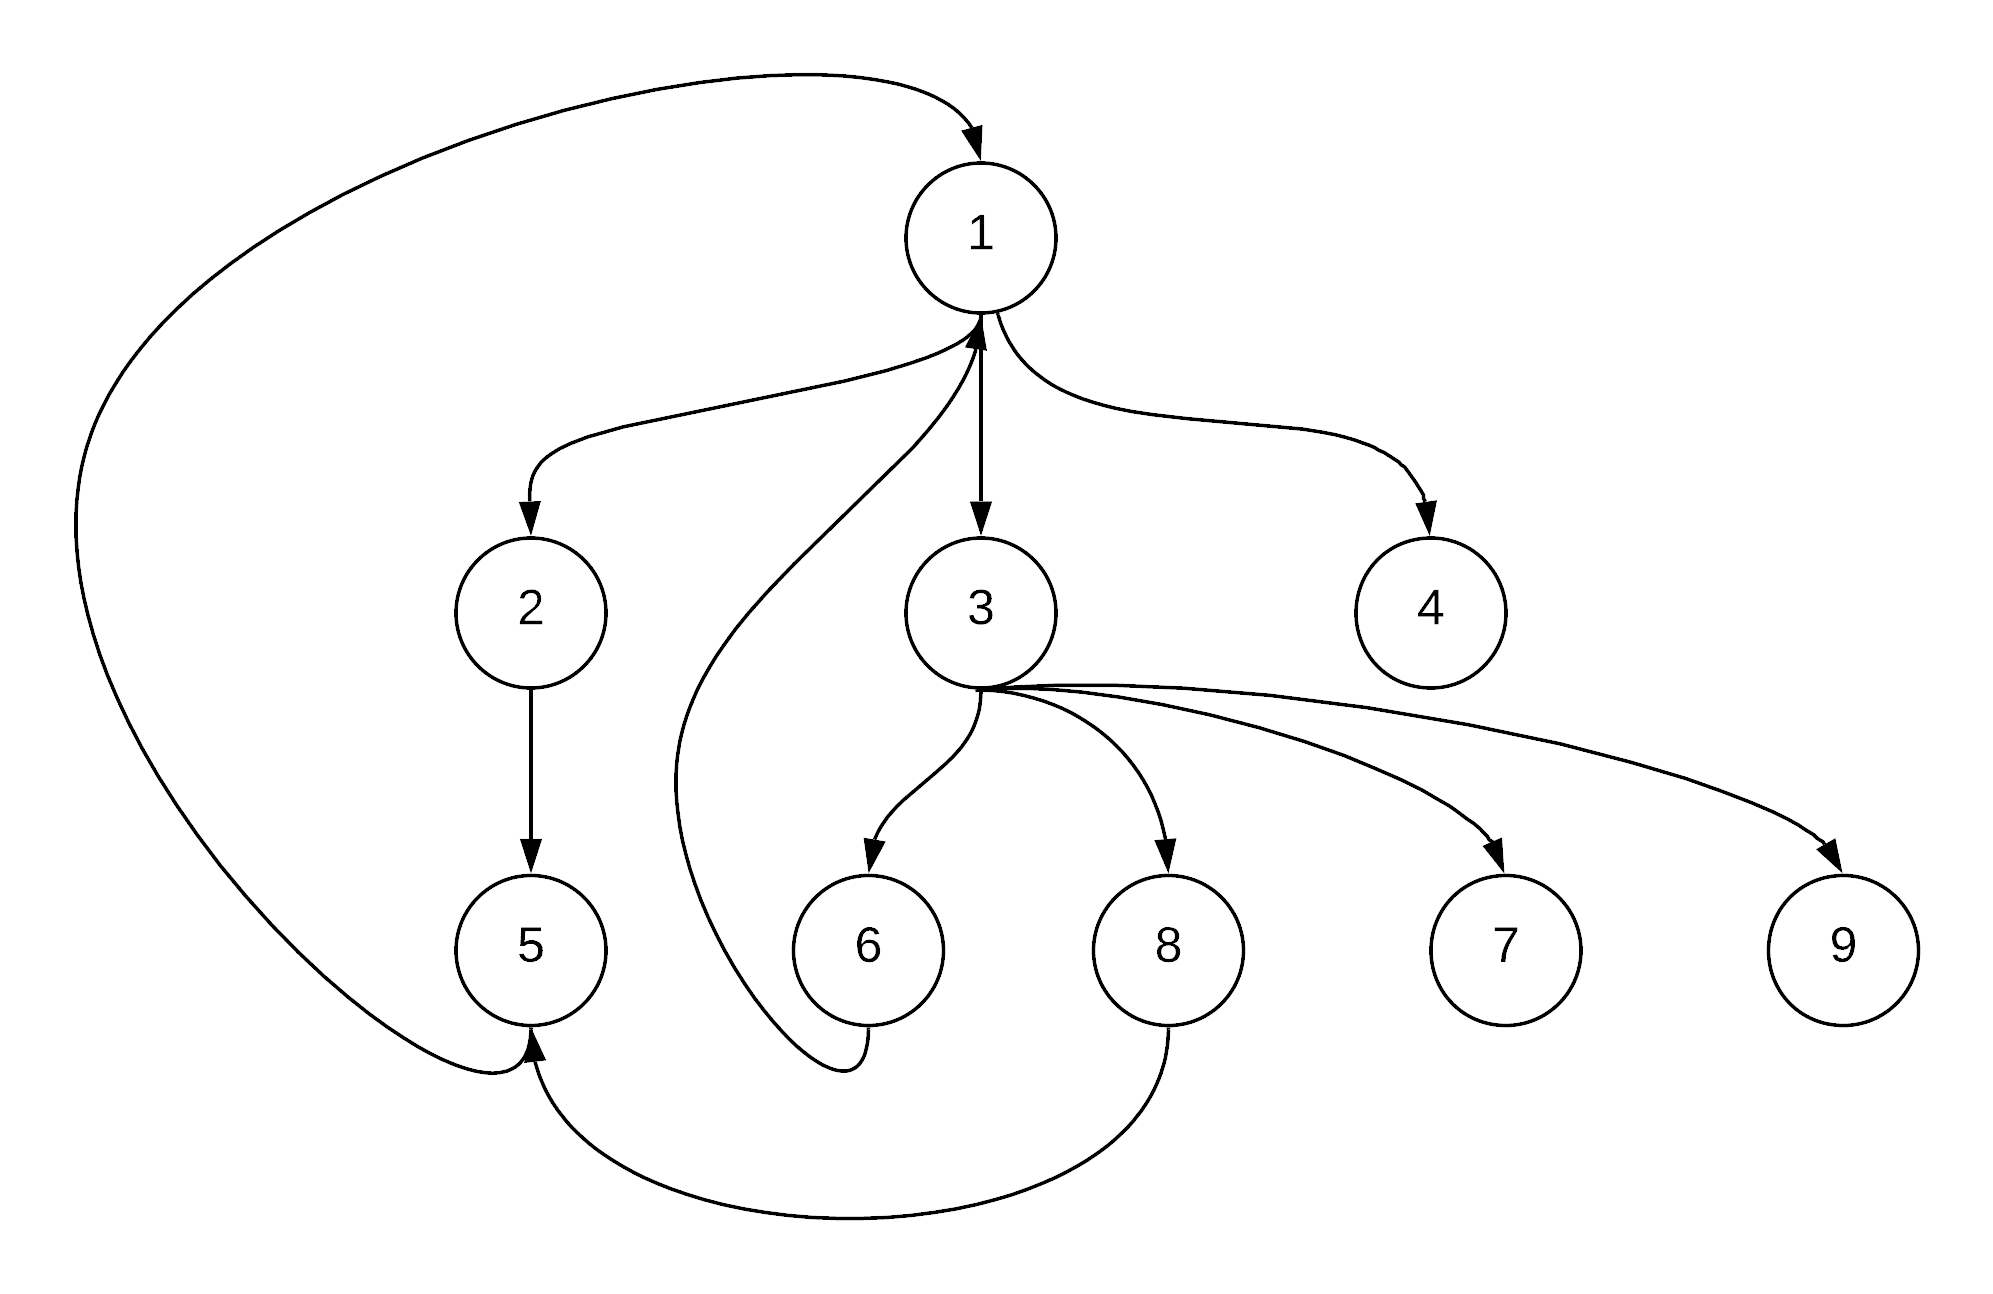
\includegraphics[scale=0.15]{graph_PPK.png}
\caption{Przykład grafu utworzonego dla danych: \newline \texttt{1->2,2->5,5->1,1->3,6->1,3->7,3->9,1->4, 3->6, 3->8, 8->5}}
\label{fig:graf}
\end{figure} 

\newpage
\subsection{Algorytmy}
Program wykorzystuje listy podwieszane do przechowywania list sąsiedztwa. Następnie wykorzystywany jest algorytm DFS do znalezienia ścieżek, a dokładniej wariant tego algorytmu, który wyszukuje
wszystkie ścieżki z wierzchołka A do wierzchołka B. Podając ten sam wierzchołek jako startowy i końcowy jesteśmy w stanie otrzymać wszystkie cykle prowadzące do danego wierzchołka. 
Algorytm DFS, czyli Depth First Search, działa w następujący sposób \cite{podstawoweAlgorytmy}: najpierw oznacza wierzchołek początkowy jako odwiedzony, odkłada go na stos,
a następnie dla każdego sąsiada wierzchołka z listy sąsiedztwa, który nie jest odwiedzony, wywołuje rekurencyjnie tę funkcję z danym elementem jako wierzchołkiem początkowym. W przeciwnym
wypadku następuje sprawdzenie, czy dany wierzchołek jest wierzchołkem końcowym. Jeżeli tak to następuje wypisanie stosu. Po przetworzeniu wszystkich wierzchołków z listy sąsiedztwa
następuje zdjęcie ze stosu elementu na jego szczycie.

Złożoność obliczeniowa \cite{podstawoweAlgorytmy} tego algorytmu wynosi $O(\|V\|+\|E\|)$, gdzie $V$ -- liczba wierzchołków, $E$ -- liczba krawędzi.
%\begin{figure}
%\centering
%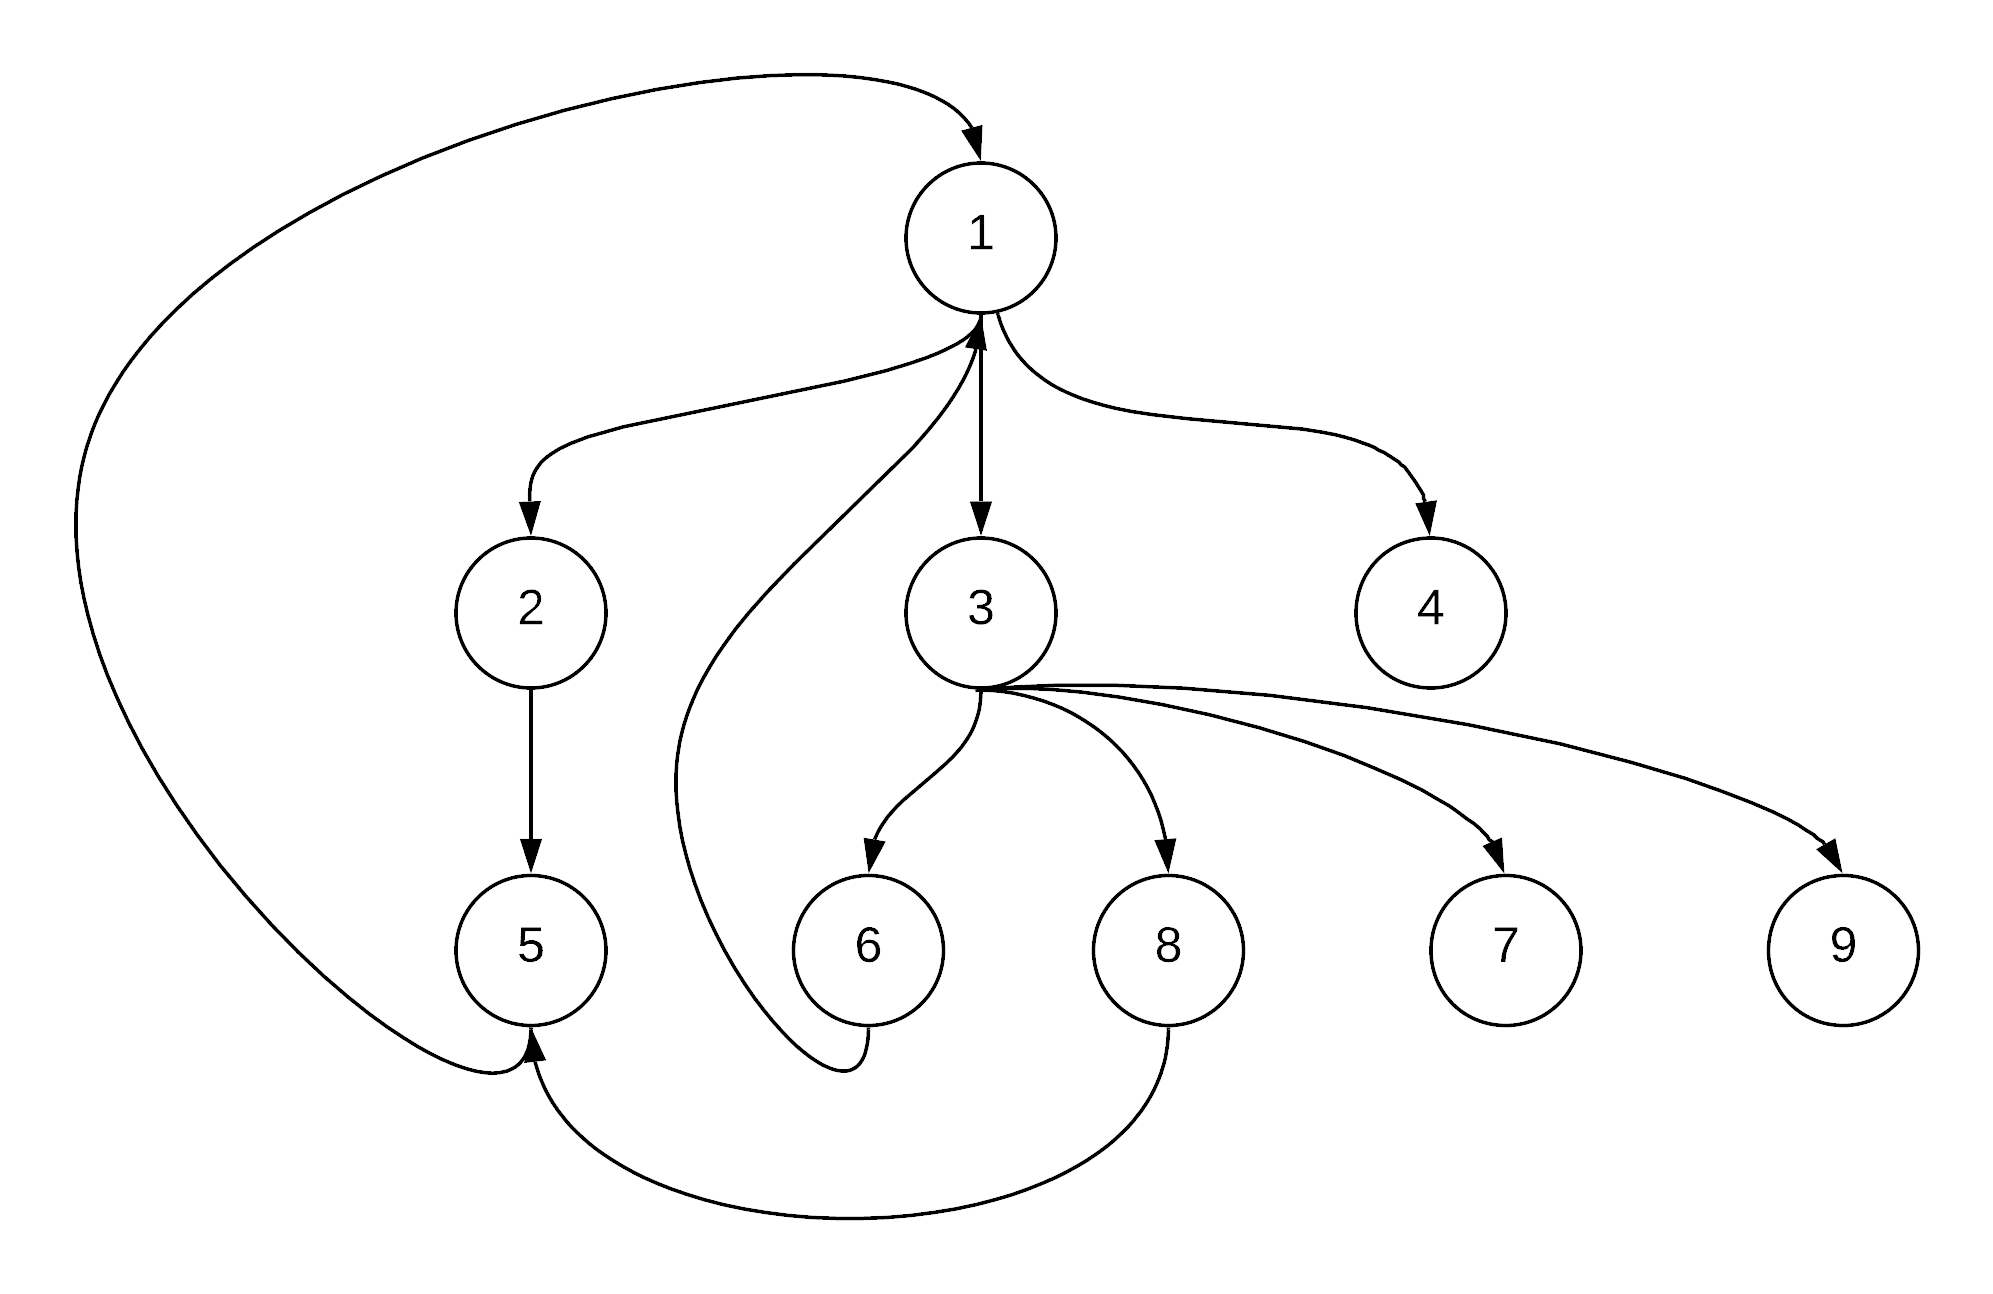
\includegraphics[scale=0.2]{graph_PPK.png}
%\caption{Przykład grafu utworzonego dla danych: \texttt{1->2,2->5,5->1,1->3,6->1,3->7,3->9,1->4, 3->6, 3->8, 8->5, 8->10, 10->10, 12-> 11, 10->11, 11->12}}
%\label{fig:graf}
%\end{figure} 

%%%%%%%%%%%%%%%%%%%%%%%%%%%%%%%%%%%%%%%%%%%%%%%%%%%%%%%%%%%%%%%%%%%%%%%%%
\section{Specyfikacja zewnętrzna}
\label{sec:sp:zewnetrzna}
Program jest uruchamiany z linii komend. Należy przekazać flagi z odpowiednimi argumentami (plik wejściowy i wyjściowy), np dla systemów UNIX:
\begin{verbatim}
./program -g wejscie -c wyjscie
./program -c cykle -g graf
\end{verbatim}
Pliki wejściowe mogą, lecz nie muszą posiadać rozszerzenia. Powinny to być pliki tekstowe, o następującej składni:
\begin{verbatim}
	<wierzcholek_startowy>-><wierzcholek_koncowy>,...
\end{verbatim} 
Uruchomienie programu z parametrem \texttt{-h}
\begin{verbatim}
program -h
\end{verbatim}
powoduje wyświetlenie krótkiej pomocy. Uruchomienie programu z nieprawidłowymi parametrami nie powoduje żadnego działania.

Podanie nieprawidłowej nazwy pliku lub brak jej podania powoduje wyświetlenie następującego błędu:
\begin{verbatim}
Błąd: nie znaleziono pliku!
\end{verbatim}

Brak podania nazwy pliku wyjściowego powoduje wyświetlenie nastepującego błędu:

\begin{verbatim}
Brak pliku wyjściowego...!
\end{verbatim}


%%%%%%%%%%%%%%%%%%%%%%%%%%%%%%%%%%%%%%%%%%%%%%%%%%%%%%%%%%%%%%%%%%%%%%%%%
\section{Specyfikacja wewnętrzna}\label{sec:sp-wew}
Program został wykonany w oparciu o paradygmat strukturalny. Rozdzielono także interfejs (komunikacja z użytkownikiem) od logiki aplikacji (wyznaczanie cykli).

\subsection{Ogólna struktura programu}
W funkcji głównej najpierw inicjowane są potrzebne zmienne i struktury. Wpierw deklarowane są zmienne typu \texttt{string} o nazwach: 
\texttt{NPlikuWej} oraz \texttt{NPlikuWyj}. Służą one do przechowywania nazw plików, na których ma operować program.
Następnie inicjowana jest struktura \texttt{ojciec} o nazwie \texttt{graf}. Słuzy ona do przechowywania reprezentacji grafu, pobranego z pliku.

Później pobrane zostają argumenty programu. Po sprawdzeniu poprawności argumentów wywołana zostaje funkcja $wczytaj \textunderscore graf$. Sprawdza ona czy plik istnieje, jeżeli nie, zwróci ona stosowny
komunikat oraz zakończy program. W przeciwnym przypadku korzystając z pomocniczych funkcji: $wyszukaj \textunderscore ojca$, $dodaj \textunderscore ojca$, $dodaj \textunderscore syna$, $dodaj \textunderscore dane$ dane zostaną wczytane do pamięci programu.

Po wczytaniu danych tworzony jest stos typu \texttt{wierzcholek} o nazwie \texttt{test}. Służy on do przechowywania stosu pomiędzy kolejnymi wywołaniami rekurencyjnymi funkcji $DFS$.
Następnie dla każdego wierzchołka jest wywoływana funkcja $DFS$, która analizuje algorytmem DFS podany graf oraz wypisuje znalezione cykle do pliku oraz na wyjście \texttt{STDERR}. Zamyka także plik wyjściowy
po zakończeniu wypisywania do niego.

Ostatnie zostają wywołane przeładowane funkcje $usun$ usuwające stos oraz graf z pamięci oraz zamknięty zostaje plik wyjściowy.
Następnie program kończy swoją pracę.

\subsection{Szczegółowy opis typów i funkcji}

Szczegółowy opis typów i funkcji zawarty jest w załączniku.

\section{Testowanie}
Program został sprawdzony dla róznych grafów skierowanych zawierających, lub nie zawierających cykli. Pliki niezgodne ze specyfikacją są nieobsługiwane. Plik pusty powoduje utworzenie pliku wyjściowego z informacją o braku cykli.
Dla grafów acyklicznych także zwrócona zostanie informacja o braku cykli. Aplikacja została przetesowana także dla danych skrajnych, niestety nie byłem w stanie napisać generatora losowego grafów, który
generowałby interesujące przypadki, ponieważ rzadko w takich grafach zdarzały się cykle.

Program nie zawiera wycieków pamięci, co zostało sprawdzone narzędziem \texttt{valgrind} dostępnym z poziomu domyślnego menadżera pakietów dla systemu Ubuntu 19.10.

\section{Uzyskane wyniki}
Program zwraca opis cykli zaczynających się z każdego wierzchołka. W szczególności program zwróci ten sam cykl dla wszystkich wierzchołków cyklu, lecz zaczynający się w innym punkcie. Przykład: dla
danych \texttt{2->3,3->2} wypisane zostaną cykle: \texttt{2->3->2} oraz \texttt{3->2->3}. Postanowiłem zaimplementować wypisywanie cykli w ten sposób aby podkreślić, że cykl może zaczynać i kończyć się
w dowolnym wierzchołku cyklu.
\section{Wnioski}
Problem wyszukiwania cykli w grafie sprawił mi małe kłopoty koncepcyjne dot. zastosowania algorytmu DFS do wyszukiwania ścieżki w grafie. Najbardziej wymagającą częścią projektu było dla mnie
jednak zaimplementowanie wczytywania danych i obsługa wyjątków. Niestety nadal nie udało mi się zaimplementować sprawdzania poprawności wczytywanych danych, ponieważ nie potrafię wymyślić zgrabnego
rozwiązania tego problemu, dlatego też mój program zakłada poprawność danych wejściowych.

\subsection{Opinie}
Wykłady były prowadzone bardzo ciekawie, poruszane zagadnienia były interesujące i życiowe. 'Live coding' także jest ciekawym doświadczeniem podczas wykładu, które bardzo doceniłem, ponieważ o wiele łatwiej było mi przyswoić materiał. Przypadła mi do gustu także metoda prowadzenia ćwiczeń na bazie "tasków", gdzie na początku zajęć od razu wiadomo, co
trzeba osiągnąć.

\begin{filecontents}{bibliografia.bib}
@article{podstawoweAlgorytmy,
	author = {Marcin Andrychowicz, Tomasz Kulczyński, Błażej Osiński},
	publisher = {Warszawska Wyższa Szkoła Informatyki},
	year = {2010},
	title = {Przegl\k{a}d podstawowych algorytm\'{o}w}

}
\end{filecontents}

\newpage

\bibliographystyle{plplain}
\bibliography{bibliografia}

 
\newpage

\rule{0cm}{0cm}

\vfill

\begin{center}
\Huge\bfseries Dodatek\\Szczegółowy opis typów i~funkcji\par
\end{center}

\vfill 

\rule{0cm}{0cm}

\end{document}
% Koniec wieńczy dzieło.
